\documentclass{beamer}
\usetheme{Madrid}

\usepackage{amsmath}
\usepackage{amssymb}
\usepackage{graphicx}
\usepackage{booktabs}

\title[Financial Goal Planner]{Financial Goal Planner: An AI-Driven Goal-Based Investment Planning and Risk-Aware Recommendation System}
\author[Group 5]{Amarthya Regimon Joseph \and Aswin P \and Athira Raj \and Haleema S}
\institute[CSE A]{Department of Computer Science and Engineering \\ CAPE College of Engineering Alappuzha \\ \vspace{0.3cm} \small \textbf{Under the guidance of:} \\ Mr. Siju Koshy \\ \footnotesize Department of Computer Science and Engineering}
\date{\today}

\begin{document}

% ---------- Title ----------
\begin{frame}
\titlepage
\end{frame}

% ---------- Contents ----------
\begin{frame}{Contents}
\tableofcontents
\end{frame}

% ================= ABSTRACT =================
\section{Introduction}

\begin{frame}{Introduction}
\small
This project proposes a \textbf{mobile application} that recommends personalized savings plans and investment allocations across mutual funds, equity, and debt instruments based on a user's financial goal, horizon, and risk profile

\medskip
The system aims to provide adaptive, risk-aware, and horizon-sensitive investment guidance through a mobile-first interface.
\end{frame}

% ================= PROBLEM STATEMENT =================
\section{Problem Statement}

\begin{frame}{Problem Statement}
\small
Individuals planning for financial goals -- such as retirement, a child's education, or purchasing a vehicle -- face difficulty determining \textbf{how much to save, for how long, and where to invest}, because the appropriate level of investment risk depends heavily on the goal's remaining time horizon.
\end{frame}

% ================= OBJECTIVE =================
\section{Objectives}

\begin{frame}{Objectives}
\begin{enumerate}
    \item To design a mobile application that allows users to define financial goals with a target amount and time horizon.
    \item To build a recommendation engine that dynamically adjusts asset allocation across mutual funds, equity, and debt instruments.
    \item To provide an intuitive mobile dashboard for tracking goal progress, required SIP contributions, and recommended portfolio adjustments over time.
\end{enumerate}
\end{frame}

% ================= LITERATURE REVIEW =================
\section{Literature Review}

% --- SLIDE 1 ---
\begin{frame}{Literature Summary (1/2)}
    \tiny
    \centering
    \begin{tabular}{p{0.5cm} p{2cm} p{4cm} p{2.5cm} c}
        \toprule
        \textbf{Ref} & \textbf{Author(s)} & \textbf{Title} & \textbf{Journal} & \textbf{Year} \\
        \midrule
        1 & Karzanov et al. & Regret-Optimized Portfolio Enhancement [BASE PAPER] & arXiv & 2025 \\
        2 & Dhashanamoorthi et al. & AI-driven robo-advisors on personal financial mgmt & Int. J. of Sci. and Research & 2024 \\
        3 & Sunilkumar & AI Revolution in Wealth Management & J. of Info Systems Eng. & 2025 \\
        4 & Ansari et al. & Multifaceted Approach to Stock Market Trading Using RL & IEEE Access & 2024 \\
        5 & Sattar et al. & RMS-Driven Deep RL for Optimized Portfolio Management & IEEE Access & 2025 \\
        6 & Yin \& Guo & Complex forecasting via chain-of-thought of LLMs & Science Direct & 2025 \\
        7 & Benhamou et al. & Detecting and adapting to crisis pattern with context DRL & arXiv & 2020 \\
        8 & Samanta et al. & Effectiveness of SIP Investment Among Retail Investors & Int. J. for Novel Research & 2024 \\
        9 & Kanagaraj et al. & Potential of AI in personal financial planning & arXiv & 2024 \\
        10 & Boaretto \& Medeiros & Forecasting inflation using disaggregates and ML & arXiv & 2023 \\
        11 & Solanki \& Jha & GAF-ResNet-LSTM Framework for Asset Selection & IEEE Access & 2025 \\
        12 & Kevin \& Yugopuspito & Hybrid LSTM and PPO Networks for Portfolio Optimization & arXiv & 2025 \\
        \bottomrule
    \end{tabular}
\end{frame}

% --- SLIDE 2 ---
\begin{frame}{Literature Summary (2/2)}
    \tiny
    \centering
    \begin{tabular}{p{0.5cm} p{2cm} p{4cm} p{2.5cm} c}
        \toprule
        \textbf{Ref} & \textbf{Author(s)} & \textbf{Title} & \textbf{Journal} & \textbf{Year} \\
        \midrule
        13 & Olamijuwon \& Zouo & ML in budget forecasting for corporate finance & Open Access Research & 2024 \\
        14 & Spadea \& Seneviratne & Parallel and Multi-Stage Knowledge Graph Retrieval & arXiv & 2025 \\
        15 & Patra et al. & AI-Driven Goal Based Financial Planning System & Rademics Research Inst. & 2025 \\
        16 & Lwele et al. & Risk-Aware Deep RL for Dynamic Portfolio Optimization & arXiv & 2025 \\
        17 & Gaspar \& Oliveira & Robo Advising and Investor Profiling & MDPI & 2024 \\
        18 & Shetty et al. & Robo-advisors in financial services & Science Direct & 2026 \\
        19 & Kofman & Scoring the Ethics of AI Robo-Advice & J. of Business Ethics & 2025 \\
        20 & Lamukanyani et al. & Sentiment-Aware Portfolio Optimization (CVaR-Based) & IEEE Access & 2025 \\
        21 & Ahn \& Kang & Simul-RL Portfolio Framework: BSM and RL & IEEE Access & 2025 \\
        22 & Pereguda et al. & Impact of the Digital Economy on Investment Portfolio Mgmt & Eastern Euro. Union & 2024 \\
        23 & Kulkarni et al. & Role of robo-advisors in behavioural finance & Cogent OA & 2020 \\
        24 & Enkhsaikhan \& Jo & Uncertainty-Aware RL for Portfolio Optimization & IEEE Access & 2024 \\
        \bottomrule
    \end{tabular}
\end{frame}

\begin{frame}{Literature Review (1/24): Regret-Optimized Portfolio Enhancement through DRL and Future Looking Rewards}
\small
\textbf{2025 -- Base Paper}
\begin{itemize}
    \item \textbf{Relation:} This is the base paper -- our project directly adapts its regret-optimized, future-looking reward formulation for goal-based, horizon-sensitive asset allocation.
    \item \textbf{Methodology:} PPO-based DRL framework for dynamic portfolio rebalancing using a regret-based reward (relative to a 60/40 benchmark) combined with a future-looking (forward-horizon) reward component; evaluated via Sharpe ratio and maximum drawdown.
\end{itemize}
\end{frame}

\begin{frame}{Literature Review (2/24): AI-driven robo-advisors on personal financial management and investment strategies}
\small
\textbf{2024}
\begin{itemize}
    \item \textbf{Relation:} Establishes the general case for AI-driven personalized investment advice that our app builds on, but uses no RL-based reward design.
    \item \textbf{Methodology:} Conceptual/survey-style analysis of how robo-advisors use algorithms and ML on market and client data to create tailored, automated investment plans.
\end{itemize}
\end{frame}

\begin{frame}{Literature Review (3/24): AI Revolution in Wealth Management: Applications and Horizons}
\small
\textbf{2025}
\begin{itemize}
    \item \textbf{Relation:} Provides industry-level context on AI adoption in wealth management, motivating the case for an AI-driven planning app, though not a DRL-based technical contribution.
    \item \textbf{Methodology:} Industry-perspective review discussing AI applications (compliance automation, personalization, back-office automation) in wealth management.
\end{itemize}
\end{frame}

\begin{frame}{Literature Review (4/24): A Multifaceted Approach to Stock Market Trading Using Reinforcement Learning}
\small
\textbf{2024}
\begin{itemize}
    \item \textbf{Relation:} Shares the RL-for-finance foundation with the base paper, but focuses on multi-stock trading rather than goal-based portfolio allocation.
    \item \textbf{Methodology:} Uses Advantage Actor-Critic (A2C) and Deep Deterministic Policy Gradient (DDPG) with a novel risk-aware reward (PSR) combining technical and fundamental indicators; validated on 30 Dow Jones stocks.
\end{itemize}
\end{frame}

\begin{frame}{Literature Review (5/24): A Novel RMS-Driven Deep RL for Optimized Portfolio Management in Stock Trading}
\small
\textbf{2025}
\begin{itemize}
    \item \textbf{Relation:} Closely related to the base paper's risk-aware reward design philosophy -- both incorporate drawdown-based rewards, though this paper adds sentiment rather than regret/future-looking terms.
    \item \textbf{Methodology:} Proposes PPO\_RMS, A2C\_RMS, and DDPG\_RMS models combining earnings-report data, Max Drawdown-based rewards, and sentiment indicators (RMS); DDPG\_RMS outperforms the DJI benchmark.
\end{itemize}
\end{frame}

\begin{frame}{Literature Review (6/24): Complex forecasting and investment strategy optimization via chain-of-thought of LLMs}
\small
\textbf{2025}
\begin{itemize}
    \item \textbf{Relation:} Explores an alternative (LLM-based) path to investment decision-making, contrasting with the base paper's RL-based approach; useful for comparing reasoning-driven vs. reward-driven strategies.
    \item \textbf{Methodology:} Applies chain-of-thought (CoT) prompting with ChatGPT-4.0 on anonymized financial statements of 608 Chinese A-share firms (2010--2023) to predict earnings direction and backtest a trading strategy.
\end{itemize}
\end{frame}

\begin{frame}{Literature Review (7/24): Detecting and adapting to crisis pattern with context based DRL}
\small
\textbf{2020}
\begin{itemize}
    \item \textbf{Relation:} An alternative robustness strategy to the base paper -- uses contextual macro features instead of regret/future-looking reward shaping to handle adverse market regimes.
    \item \textbf{Methodology:} Two sub-network DRL architecture; one network processes past strategy performance/volatility, the other processes macro-context features (risk aversion, economic surprise index, cross-asset correlation), with adversarial training for robustness.
\end{itemize}
\end{frame}

\begin{frame}{Literature Review (8/24): Effectiveness of SIP Investment Among Retail Investors in Jharkhand}
\small
\textbf{2024}
\begin{itemize}
    \item \textbf{Relation:} Grounds our project's Indian retail-investor context and validates SIP as the primary savings vehicle our app should recommend for goal-based plans.
    \item \textbf{Methodology:} Primary survey-based study assessing awareness, adoption, and perceived effectiveness of Systematic Investment Plans (SIPs) among retail investors in the Jharkhand region.
\end{itemize}
\end{frame}

\begin{frame}{Literature Review (9/24): Exploring the potential of AI in personal financial planning and advisory services}
\small
\textbf{2024}
\begin{itemize}
    \item \textbf{Relation:} Supports the motivation for our app's AI-driven advisory features (automation, predictive analytics, risk profiling), though it is a conceptual/industry piece rather than a DRL contribution.
    \item \textbf{Methodology:} Discussion-style analysis of AI use cases (automation, predictive analytics, risk assessment) in personal financial planning and advisory workflows.
\end{itemize}
\end{frame}

\begin{frame}{Literature Review (10/24): Forecasting inflation using disaggregates and machine learning}
\small
\textbf{2023}
\begin{itemize}
    \item \textbf{Relation:} Relevant to our goal-cost projection module -- our app must inflate future goal costs (e.g. education, car price) accurately, and this paper's ML forecasting approach can inform that sub-module.
    \item \textbf{Methodology:} Aggregates disaggregated (bottom-up) inflation forecasts using linear and nonlinear ML models, applied to Brazilian inflation data, and compares against direct aggregate forecasting.
\end{itemize}
\end{frame}

\begin{frame}{Literature Review (11/24): From Time Series to Images: A GAF-ResNet-LSTM Framework for Portfolio Optimization}
\small
\textbf{2025}
\begin{itemize}
    \item \textbf{Relation:} An alternative deep-learning approach (image-based) to asset selection that could complement our recommendation engine's fund-selection stage, contrasting with the base paper's pure RL approach.
    \item \textbf{Methodology:} Converts price sequences into Gramian Angular Field (GAF) images, extracts spatial features via ResNet and temporal features via LSTM, then applies nested clustered optimization (NCO); validated on NIFTY 50 constituents.
\end{itemize}
\end{frame}

\begin{frame}{Literature Review (12/24): Hybrid LSTM and PPO Networks for Dynamic Portfolio Optimization}
\small
\textbf{2025}
\begin{itemize}
    \item \textbf{Relation:} Directly extends the base paper's PPO approach with a forecasting layer -- a natural reference for a possible future enhancement to our recommendation engine.
    \item \textbf{Methodology:} Combines an LSTM forecasting sub-module with a PPO-based allocation agent so decisions are informed by learned temporal price patterns.
\end{itemize}
\end{frame}

\begin{frame}{Literature Review (13/24): Machine learning in budget forecasting for corporate finance}
\small
\textbf{2024}
\begin{itemize}
    \item \textbf{Relation:} While corporate-focused, the proposed ML-driven forecasting architecture is conceptually transferable to our app's personal budget/savings-capacity forecasting module.
    \item \textbf{Methodology:} Conceptual model integrating regression, time-series analysis, and neural networks into a budget forecasting architecture for corporate financial planning.
\end{itemize}
\end{frame}

\begin{frame}{Literature Review (14/24): Parallel and Multi-Stage Knowledge Graph Retrieval for Financial Asset Recommendations}
\small
\textbf{2025}
\begin{itemize}
    \item \textbf{Relation:} Closely relevant to our app's recommendation engine design -- shows how to align recommendations with investor behavior, complementing the base paper's reward-based personalization.
    \item \textbf{Methodology:} Knowledge-graph-based retrieval system evaluated on the FAR-Trans dataset, using strict temporal cutoffs to avoid data leakage when generating behaviorally-aligned asset recommendations.
\end{itemize}
\end{frame}

\begin{frame}{Literature Review (15/24): Regret-Optimized Portfolio Enhancement through DRL and Future Looking Rewards}
\small
\textbf{2025 -- Base Paper}
\begin{itemize}
    \item \textbf{Relation:} This is the base paper -- our project directly adapts its regret-optimized, future-looking reward formulation for goal-based, horizon-sensitive asset allocation.
    \item \textbf{Methodology:} PPO-based DRL framework for dynamic portfolio rebalancing using a regret-based reward (relative to a 60/40 benchmark) combined with a future-looking (forward-horizon) reward component; evaluated via Sharpe ratio and maximum drawdown.
\end{itemize}
\end{frame}

\begin{frame}{Literature Review (16/24): Risk-Aware Deep Reinforcement Learning for Dynamic Portfolio Optimization}
\small
\textbf{2025}
\begin{itemize}
    \item \textbf{Relation:} Closest methodological sibling to the base paper -- both use PPO with risk-sensitive rewards, useful for comparing regret-based vs. Sharpe-based reward design in our engine.
    \item \textbf{Methodology:} Integrates a Sharpe-ratio-based reward with direct risk controls (maximum drawdown, volatility constraints), trained using PPO; benchmarked against mean-variance and equal-weighted portfolios.
\end{itemize}
\end{frame}

\begin{frame}{Literature Review (17/24): Robo Advising and Investor Profiling}
\small
\textbf{2024}
\begin{itemize}
    \item \textbf{Relation:} Directly relevant to our risk-profiling module -- proposes an objective, quantifiable risk measure that our app's questionnaire-based profiling could adopt instead of vague risk buckets.
    \item \textbf{Methodology:} Introduces an investor profiling method based solely on Relative Risk Aversion (RRA), deriving optimal allocations and comparing them against real robo-advisor (Riskalyze) portfolios for conservative, moderate, and aggressive profiles.
\end{itemize}
\end{frame}

\begin{frame}{Literature Review (18/24): Robo-advisors in financial services: Redefining wealth management in the age of AI}
\small
\textbf{2026}
\begin{itemize}
    \item \textbf{Relation:} Provides a structured typology of robo-advisor institutional forms, useful for positioning our app's design choices within the broader robo-advisory landscape.
    \item \textbf{Methodology:} Conceptual model (grounded in Dubin's theory-building framework) categorizing robo-advisors into Wealth Management Firm, Regulatory, and Personal types, linking institutional design to return maximization, risk minimization, and financial inclusion outcomes.
\end{itemize}
\end{frame}

\begin{frame}{Literature Review (19/24): Scoring the Ethics of AI Robo-Advice: Why We Need Gateways and Ratings}
\small
\textbf{2025}
\begin{itemize}
    \item \textbf{Relation:} Important for our project's ethical/regulatory considerations -- highlights trust and transparency issues our app must address when recommending investment allocations.
    \item \textbf{Methodology:} Proposes a regulatory framework requiring robo-advisors to clear four licensing gateways for an AI Robo-Advice License (AIRAL), followed by ongoing ethical-compliance monitoring via a balanced scorecard rating.
\end{itemize}
\end{frame}

\begin{frame}{Literature Review (20/24): Sentiment-Aware Portfolio Optimization: CVaR-Based Diversification With DRL}
\small
\textbf{2025}
\begin{itemize}
    \item \textbf{Relation:} Shares the risk-control philosophy of the base paper (CVaR vs. regret) and shows how sentiment can be incorporated into the state space, a possible future extension for our engine.
    \item \textbf{Methodology:} Uses DDPG to dynamically adjust allocations under Conditional Value-at-Risk (CVaR) constraints while incorporating FinBERT-derived sentiment scores into the state representation, accounting for transaction costs.
\end{itemize}
\end{frame}

\begin{frame}{Literature Review (21/24): Simul-RL Portfolio Framework: Black-Scholes-Merton and RL for Asset Allocation}
\small
\textbf{2025}
\begin{itemize}
    \item \textbf{Relation:} Addresses a limitation relevant to our project -- limited historical data for personal goal scenarios -- by showing how simulated data can augment RL training, unlike the base paper which relies on historical market data alone.
    \item \textbf{Methodology:} Uses Monte Carlo simulation data (grounded in the Black-Scholes-Merton model) to increase training data complexity and diversity for an RL-based asset allocation agent, addressing overfitting and limited statistical structure in real data.
\end{itemize}
\end{frame}

\begin{frame}{Literature Review (22/24): The Impact of the Digital Economy on Investment Portfolio Management}
\small
\textbf{2024/25*}
\begin{itemize}
    \item \textbf{Relation:} Provides macro-level context on how digital transformation is reshaping portfolio management practices, motivating our project's digital-first (mobile app) approach.
    \item \textbf{Methodology:} Empirical/analytical study examining how digital economy indicators relate to investment portfolio management and investor behavior in stock markets.
\end{itemize}
\end{frame}

\begin{frame}{Literature Review (23/24): The role of robo-advisors in behavioural finance, shaping investment decisions}
\small
\textbf{2020}
\begin{itemize}
    \item \textbf{Relation:} Relevant to our app's UX and risk-communication design -- highlights behavioral biases robo-advisors must account for, complementing the base paper's purely quantitative reward design.
    \item \textbf{Methodology:} Longitudinal case study examining robo-advisors through the lens of behavioural finance and their role in shaping investors' financial decision-making processes.
\end{itemize}
\end{frame}

\begin{frame}{Literature Review (24/24): Uncertainty-Aware Reinforcement Learning for Portfolio Optimization}
\small
\textbf{2024}
\begin{itemize}
    \item \textbf{Relation:} Extends the base paper's risk-awareness with explicit uncertainty quantification (Bayesian forecasting), a potential enhancement for our engine's confidence-aware recommendations.
    \item \textbf{Methodology:} Proposes the Uncertainty-Aware Markov Decision Process (UAMDP), coupling Bayesian forecasting, posterior-sampling RL (Thompson sampling), and CVaR-constrained planning; improves Sharpe ratio and roughly halves maximum drawdown vs. baselines.
\end{itemize}
\end{frame}

% ================= RESEARCH GAP =================
\section{Research Gap}

\begin{frame}{Research Gap}
\small
\begin{itemize}
    \item \textbf{Robo-advisory and AI financial planning literature} covers general AI-driven advisory concepts, investor profiling, ethics, and Indian SIP adoption -- but none integrate a \emph{dynamic, reward-shaped} recommendation engine tied to a specific goal's remaining time horizon.
    \item \textbf{No existing system combines:}
    \begin{enumerate}
        \item Goal-based horizon-aware planning (amount, deadline, inflation-adjusted target),
        \item A mobile-first, India-relevant recommendation engine spanning mutual funds, equity, and debt instruments.
    \end{enumerate}
    \item \textbf{This project's contribution:} bridging goal-based financial planning with regret-based, future-looking DRL reward shaping in a single mobile recommendation system.
\end{itemize}
\end{frame}

% ================= PROJECT PLANNING =================
\section{Project Planning}

\begin{frame}{Project Planning: Project Calendar}
\begin{figure}
    \centering
    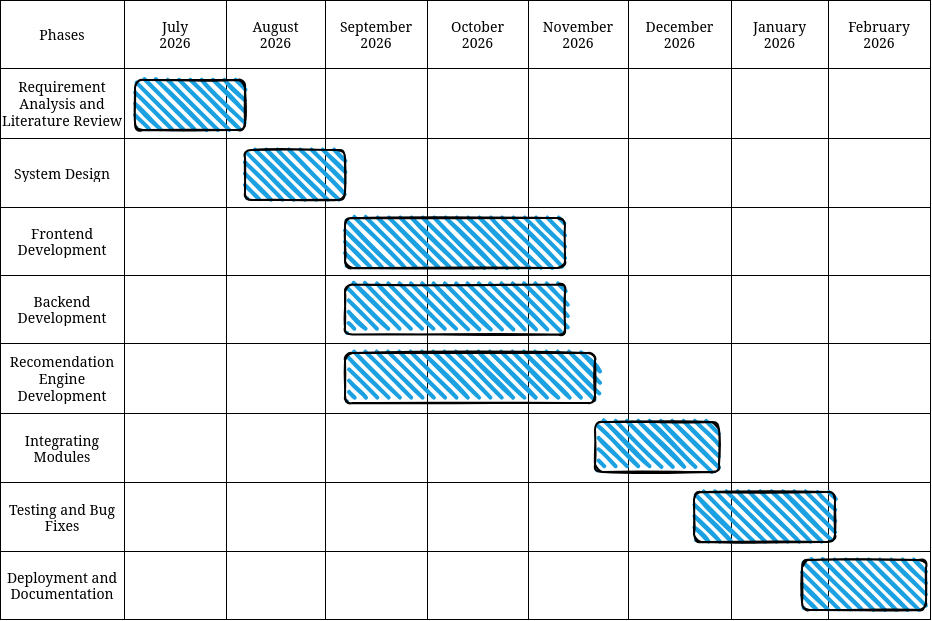
\includegraphics[width=0.95\textwidth]{project_calendar.png}
\end{figure}
\end{frame}

\begin{frame}{Project Planning: Phase-wise Timeline}
\small
\begin{itemize}
    \item \textbf{July 1 -- August 10:} Requirement analysis, literature review finalization
    \item \textbf{August 11 -- September 5:} System design -- UML diagrams, architecture
    \item \textbf{September 6 -- November 15:} Frontend Development
    \item \textbf{September 6 -- November 15:} Backend development Development
    \item \textbf{September 6 -- November 25:} Recommendation engine development \& training
    \item \textbf{November 26 -- December 25:} Integration of frontend, backend, and recommendation engine
    \item \textbf{December 21 -- February 5:} Testing, bug fixing, and evaluation against benchmarks
    \item \textbf{January 26 -- February 28:} Documentation and final presentation preparation
\end{itemize}
\end{frame}

\begin{frame}{Athira Raj --- Mobile Application \& UI/UX}
\small
\textbf{Primary:}
\begin{itemize}
    \item UI/UX architecture
    \item Mobile screens
    \item Goal creation interface
    \item Dashboard
    \item Recommendation visualization
\end{itemize}
\textbf{Supporting:}
\begin{itemize}
    \item Frontend-backend integration
    \item User testing
\end{itemize}
\end{frame}

\begin{frame}{Haleema S --- Risk Profiling \& User Modelling}
\small
\textbf{Primary:}
\begin{itemize}
    \item Risk questionnaire
    \item Risk tolerance
    \item Risk capacity
    \item Risk classification
    \item User financial profile
\end{itemize}
\textbf{Supporting:}
\begin{itemize}
    \item Risk-related literature analysis
    \item Testing different user profiles
\end{itemize}
\medskip
\end{frame}

\begin{frame}{Amarthya Regimon Joseph --- AI Recommendation \& Portfolio Allocation}
\small
\textbf{Primary:}
\begin{itemize}
    \item Recommendation engine
    \item Time-horizon analysis
    \item Asset allocation
    \item Dynamic portfolio adjustment
    \item Base paper's DRL concepts
\end{itemize}
\textbf{Supporting:}
\begin{itemize}
    \item PPO/reward mechanism study
    \item Benchmark comparison
    \item Recommendation evaluation
\end{itemize}
\medskip
\end{frame}

\begin{frame}{Aswin P --- Financial Forecasting \& Financial Computation}
\small
\textbf{Primary:}
\begin{itemize}
    \item Inflation-adjusted goal amount
    \item Future Value calculation
    \item SIP calculation
    \item Expected investment growth
    \item Goal feasibility
    \item Financial/market data processing
\end{itemize}
\textbf{Supporting:}
\begin{itemize}
    \item Forecasting model/data analysis
    \item Financial API integration
    \item Validation of financial calculations
\end{itemize}
\medskip
\end{frame}

% ================= UML DIAGRAMS =================
\section{System Architecture \& Modular Breakdown}
\begin{frame}{System Architecture}
\begin{figure}
    \centering
    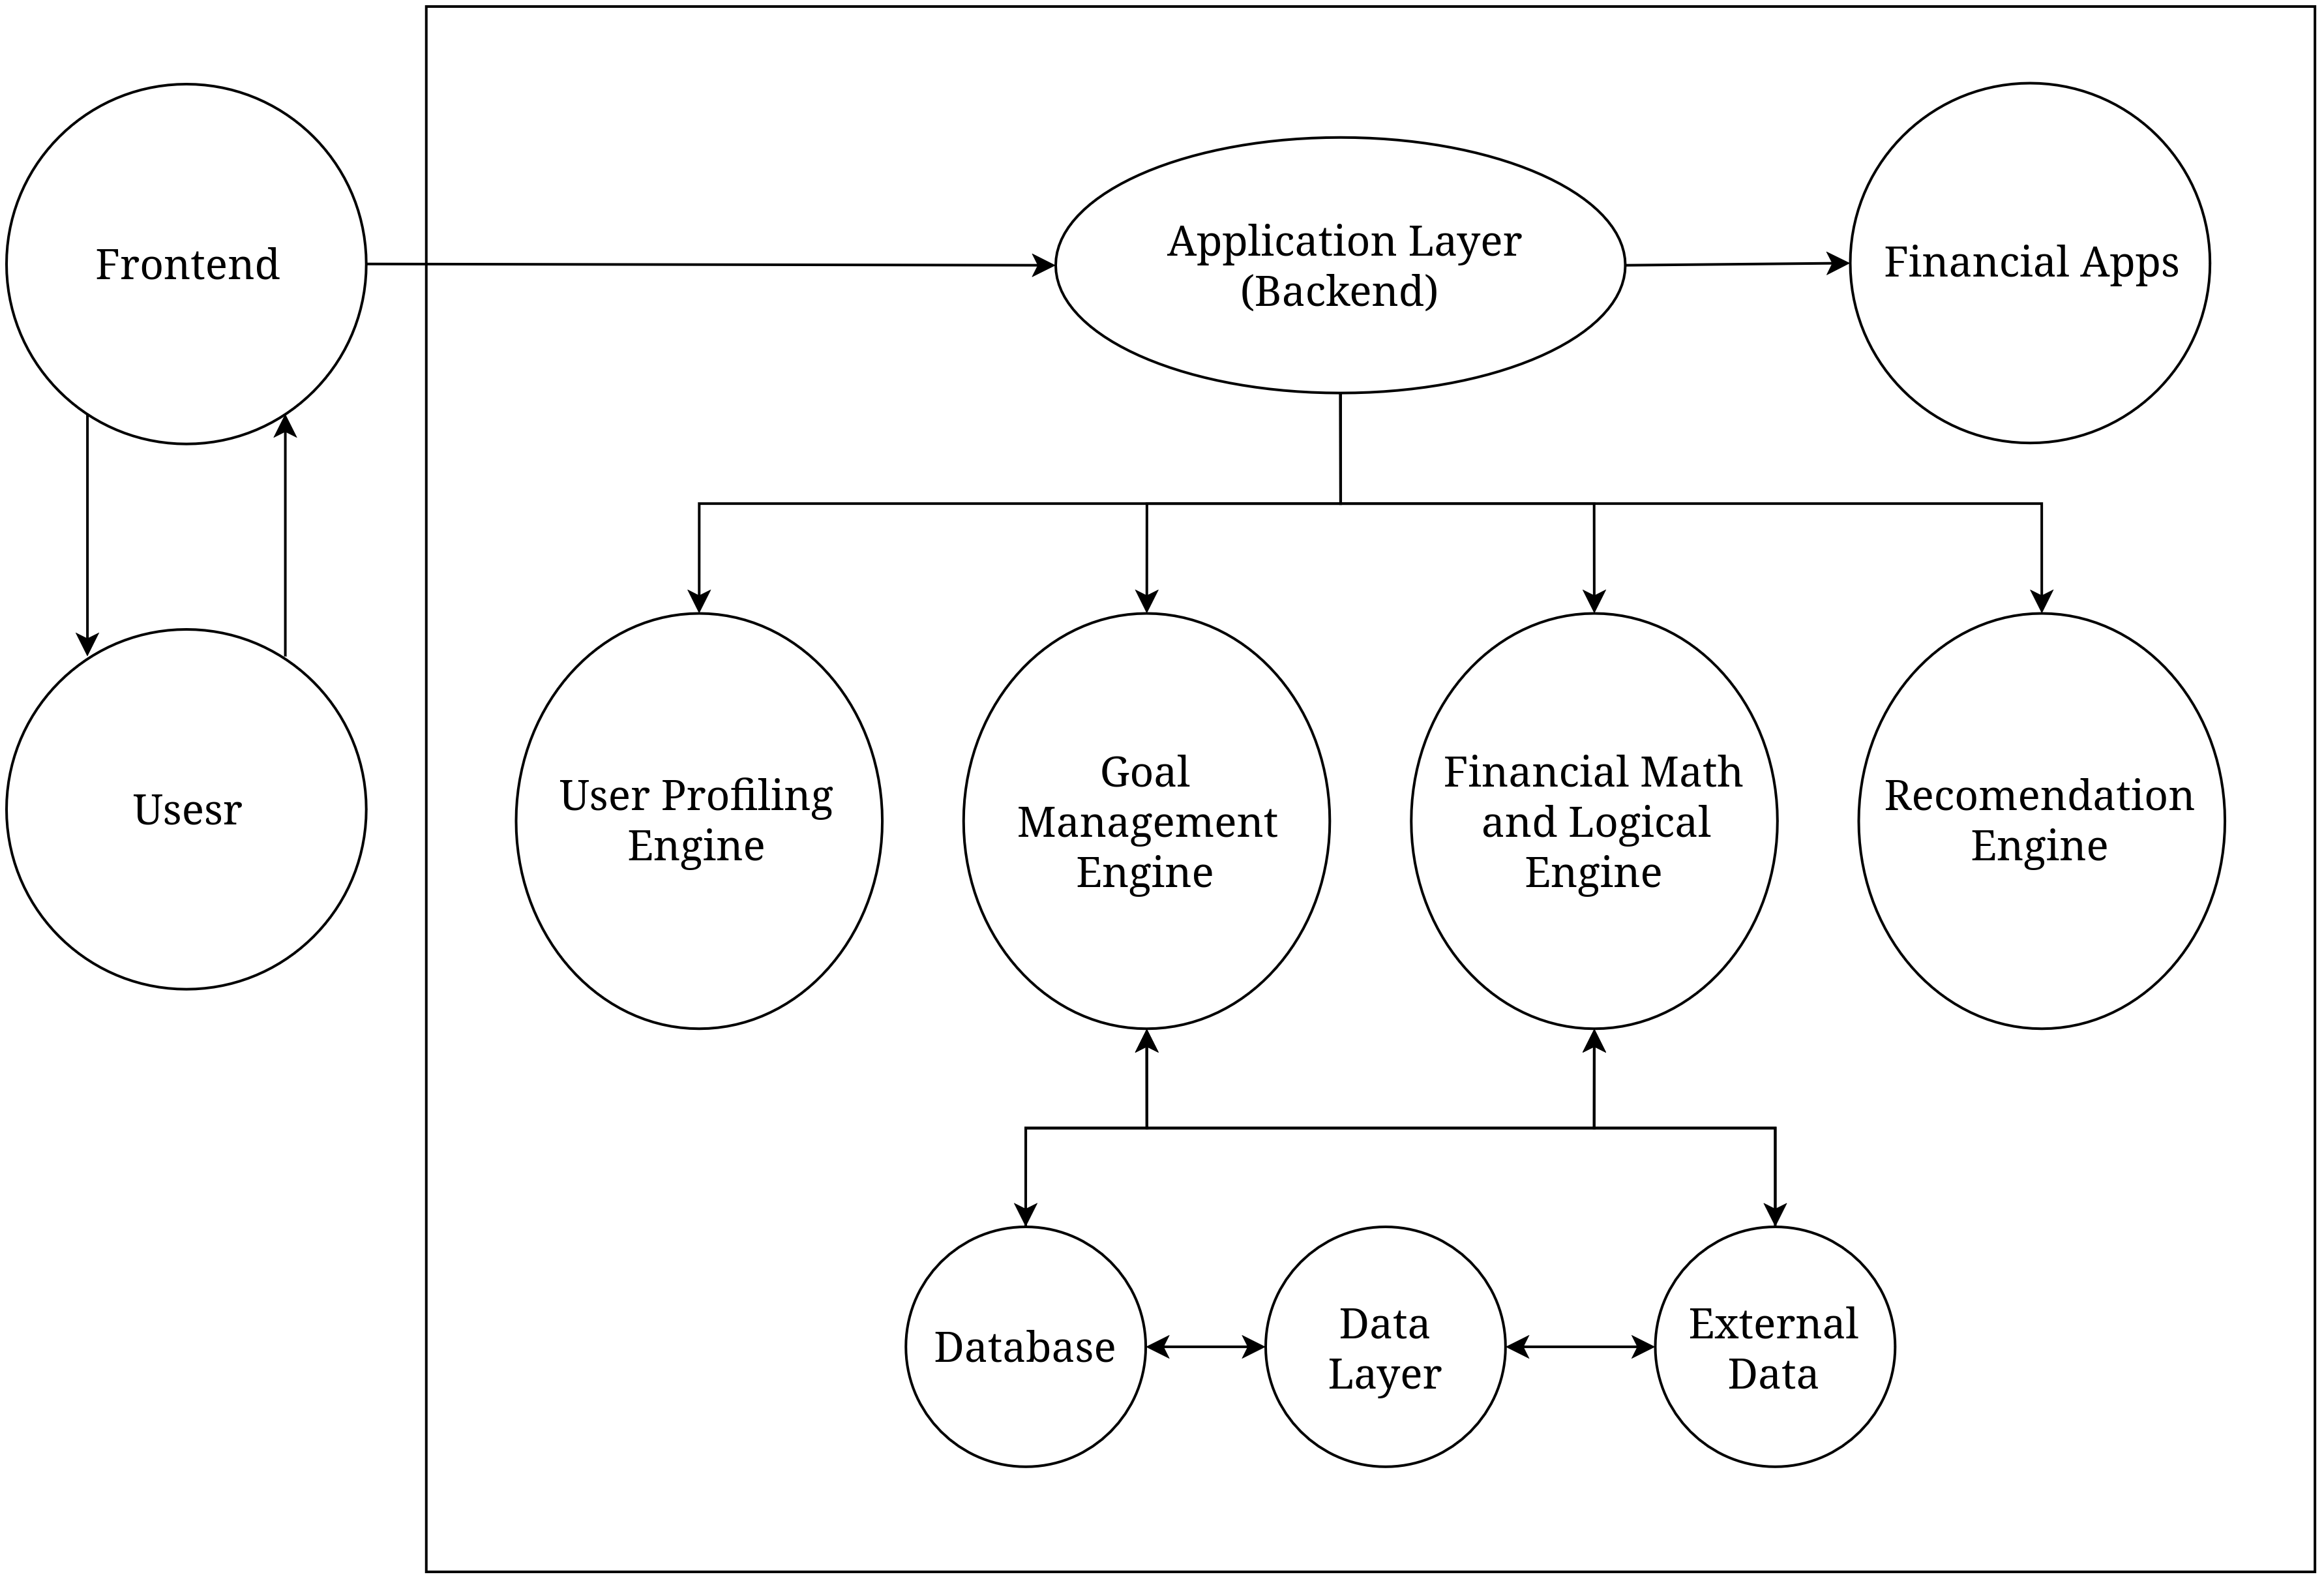
\includegraphics[width=0.85\textwidth]{system_architecture.png}
\end{figure}
\end{frame}

\begin{frame}{Modular Breakdown}
    \begin{block}{Module 1: Mobile Application \& UI/UX}
        \begin{itemize}
            \item UI/UX architecture, Mobile Screens, Recommendation visualization.
            \item Goal Creation Interface, Dashboard.
        \end{itemize}
    \end{block}
    \begin{block}{Module 2: AI Recomendation and Portfolio Allocation}
        \begin{itemize}
            \item Recomendation Engine, Time Horizon Analysis.
            \item Asset Allocation, Portfolio Reallocation.
        \end{itemize}
    \end{block}
    \begin{block}{Module 3: Risk Profiling and \& Modelling}
        \begin{itemize}
            \item Risk Quiestionaire, Risk Tolerance, Risk Capacity.
            \item Risk Classification, User financial Profile.
        \end{itemize}
    \end{block}
    \begin{block}{Module 4: Financial Forecasting \& Financial Computation}
        \begin{itemize}
            \item Inflation adjusted Goal amount, SIP Calculation.
            \item Expected Investment Growth, Market Data Processing.
        \end{itemize}
    \end{block}
\end{frame}

\section{Tools and Technologies Used}
\begin{frame}{Tools and Technologies Used}
\begin{itemize}
    \item \textbf{Frontend (Mobile App):} Flutter
    \item \textbf{Backend:} Python (FastAPI)
    \item \textbf{Database:} Supabase (Postgres)
    \item \textbf{Recommendation Engine:} Python, PyTorch / Stable-Baselines3
    \item \textbf{Version Control:} Git \& GitHub
\end{itemize}
\medskip
\end{frame}

\section{Requirements}
\begin{frame}{Functional Requirements}

\small

\begin{itemize}
    \setlength{\itemsep}{8pt}

    \item \textbf{Financial Goal Management:}
    Allow users to define financial goals with target amount and time horizon.

    \item \textbf{Risk Profiling:}
    Assess the user's risk tolerance and risk capacity to classify the user's risk profile.

    \item \textbf{Financial Calculation:}
    Calculate inflation-adjusted goal amount, required SIP contribution, and expected investment growth.

    \item \textbf{Investment Recommendation:}
    Recommend suitable allocation across mutual funds, equity, and debt instruments based on the user's goal and risk profile.

    \item \textbf{Dynamic Portfolio Adjustment:}
    Adjust asset allocation based on the remaining goal horizon, risk profile, and changing market conditions.

\end{itemize}

\end{frame}

\begin{frame}{Non-Functional Requirements}

\small

\begin{itemize}
    \setlength{\itemsep}{9pt}

    \item \textbf{Usability:}
    The application should provide a simple and intuitive mobile-first interface.

    \item \textbf{Performance:}
    Financial calculations and investment recommendations should be generated efficiently.

    \item \textbf{Security:}
    User personal and financial information should be securely handled and stored.

    \item \textbf{Reliability:}
    Financial calculations and recommendation results should be consistent and dependable.

    \item \textbf{Accuracy:}
    Goal calculations, SIP calculations, inflation adjustments, and portfolio recommendations should provide reliable results.

\end{itemize}

\end{frame}


% ================= CONCLUSION =================
\section{Conclusion}



\begin{frame}{Conclusion}
\small
\begin{itemize}
    \item Existing goal-based financial planning tools rely on static, rule-based risk assessment that does not adapt to a goal's remaining time horizon or evolving market conditions.
    \item The reviewed literature demonstrates strong individual advances in robo-advisory design, and behavioral/ethical considerations -- but no single system unifies these for \textbf{personal, goal-based} investment planning.
    \item This project proposes a mobile application that adapts the base paper's regret-optimized, future-looking reward mechanism to recommend dynamic investment allocations for individual financial goals.
    \item This phase 1 review establishes the problem statement, objectives, literature foundation, system design, Modular division and Technological requirements.
\end{itemize}
\end{frame}

% ================= REFERENCES =================
\section{References}

\begin{frame}[allowframebreaks]{References}
    \nocite{*}
    \bibliographystyle{ieeetr}
    \bibliography{references}
\end{frame}

\begin{frame}
\centering
\Huge Thank You
\end{frame}

\end{document}